% MAS1004 Assignment 1: long report.
%
% You fill this in with your agent, in your repository. AGENTS.md tells the
% agent how. Red text in the PDF is what still has to be replaced.
%
% - Pictures go in figures/. Copy them from results/, which is not in git.
% - Outputs go in outputs/. run.py saves what it prints in
%   results/<tag>_output.txt, and PLAN.md saves the other outputs in results/
%   with `| tee results/...`. Copy them here. \outputfile{outputs/check.txt}
%   prints a file exactly as it is. Every number in this report has to come
%   from such an output.
%
% To make the PDF: compress this folder into a zip, and on Overleaf choose
% New Project, Upload Project. Set Menu, Compiler to XeLaTeX, and Recompile.

\documentclass[11pt]{article}
\usepackage[ko]{mas1004}

\reporttitle{Assignment 1: Long report}
\studentname{\fillin{이름 입력}}
\studentid{\fillin{학번 입력}}

\begin{document}
\makeheader

% ---------------------------------------------------------------------------
\section*{Problem 1. Categories and images}

\subsection*{Why these categories}
두산 팬이며, LG·한화·키움 유니폼 사진은 지인에게 직접 촬영한 사진을 구할 수 있어 네 구단을 선택했다. 흰색과 세로 줄무늬 등 비슷한 특징을 가진 유니폼을 어떻게 구분하는지 궁금했다. 분류 범주는 두산·LG·한화·키움의 네 구단이며, 2026시즌에 착용하는 홈·원정·특별 유니폼을 모두 포함한다.

\subsection*{What I expected the model to use}
학습 전에는 팀 로고와 팀명, 팀 색상, 선수 이름·번호, 엠블럼 패치 등을 단서로 구단을 구분할 것으로 예상했다. 이는 사용자가 학습 전에 제시한 예상이며, Problem 7에서 사용자가 직접 정한 실험으로 검토할 예정이다.

\subsection*{Images per category}
각 구단 이름에 2026과 uniform을 포함한 검색어로 150장씩, 총 600장을 수집했다. 검색어에 2026을 포함했어도 이전 시즌·다른 구단·유니폼이 아닌 사진이 섞여 있었다.
\outputfile{outputs/collection_output.txt}

% ---------------------------------------------------------------------------
\section*{Problem 2. Preparing an image}

\sidebyside{figures/prepare_original.jpg}{두산 0006 원본}
           {figures/prepare_result.png}{중앙을 잘라낸 224$\times$224 입력의 색상 복원 표시}

원본 650×813 사진의 짧은 변을 256으로 축소한 뒤 중앙 224×224 영역을 잘라낸다. 이 예시에서는 모자 윗부분과 하의 아래쪽이 잘리지만 가슴 글자는 남는다. 모델은 원본 전체를 보는 것이 아니다.
\picturefile{figures/preprocessing-example.png}
\fillin{추가 확인: 유니폼 자체의 중요한 부분이 잘리는 사진을 선택하고 설명하기.}

% ---------------------------------------------------------------------------
\section*{Problem 3. First training runs}

\begin{center}\footnotesize
\resizebox{\linewidth}{!}{\begin{tabular}{llllrrrr}
\toprule
tag & start & trained & epochs & lr & trainable parameters & train acc. & test acc. \\
\midrule
run & ImageNet & all layers & 10 & 0.0001 & 11,178,564 & 99.8\% & 85.0\% \\
scratch & random & all layers & 10 & 0.0001 & 11,178,564 & 99.8\% & 53.3\% \\
frozen & ImageNet & last layer & 10 & 0.001 & 2,052 & 85.4\% & 74.2\% \\
low\_lr & ImageNet & all layers & 10 & 3e-05 & 11,178,564 & 99.8\% & 80.8\% \\
\bottomrule
\end{tabular}}
\end{center}

\picturefile{figures/run_curves.png}

기본 실험의 학습 손실은 1.0118에서 0.0081로 감소했다. 시험 손실은 초반에 크게 감소한 뒤 0.3대에서 움직였으며 마지막에는 0.3461이었다. 학습 손실 감소가 시험 성능의 지속적인 개선으로 이어지지는 않았다.

기본 실험의 최종 학습 정확도는 99.8\%, 시험 정확도는 85.0\%로 차이는 14.8\%p였다. 학습 사진에 대한 높은 정확도가 새로운 시험 사진에서도 그대로 유지되지는 않았다. 또한 이 단계의 라벨은 정제 전 검색 결과의 폴더 라벨이므로, 잘못된 라벨과 유사 사진이 포함된 결과라는 한계가 있다.

\begin{center}\picturefile[0.5\linewidth]{figures/run_confusion.png}\end{center}

기본 실험에서 가장 많이 혼동한 구단 조합은 두산과 키움이었다. 두산 폴더 사진 6장을 키움으로, 키움 폴더 사진 3장을 두산으로 예측했다.
\fillin{이 혼동이 예상과 달랐는지 사용자의 생각을 추가하기.}

ImageNet에서 출발한 기본 실험은 시험 정확도 85.0\%, 무작위 초기화 실험은 53.3\%로 31.7\%p 차이가 났다. 기존에 학습한 이미지 특징을 활용한 것이 이 데이터와 10회 학습 조건에서 유리했을 가능성이 있다. 각 설정은 한 번씩 실행했으며, 데이터 분할 seed는 같지만 모델 초기화와 배치 순서를 별도로 고정하지 않아 확률적 차이도 포함된다.

마지막 층만 학습한 실험의 시험 정확도는 74.2\%로 전체 층 학습보다 10.8\%p 낮았다. 학습 대상은 2,052개로 전체 11,178,564개의 0.0184\%였다. 사용자가 선택한 학습률 0.00003 실험은 시험 정확도 80.8\%로 기본보다 4.2\%p 낮았다. 시험 성능 정체를 보고 더 작은 학습률을 비교했지만, 이번 10회 실험에서는 개선되지 않았다. 처음부터 고정한 학습률을 비교했으며, 기존 모델을 이어 학습하거나 중간에 학습률을 바꾼 실험은 아니다.
\picturefile{figures/experiment-comparison.png}
\outputfile{outputs/run_analysis_output.txt}

\subsection*{scratch}
\picturefile{figures/scratch_curves.png}
\begin{center}\picturefile[0.6\linewidth]{figures/scratch_confusion.png}\end{center}
\subsection*{frozen}
\picturefile{figures/frozen_curves.png}
\begin{center}\picturefile[0.6\linewidth]{figures/frozen_confusion.png}\end{center}
\subsection*{low\_lr}
\picturefile{figures/low_lr_curves.png}
\begin{center}\picturefile[0.6\linewidth]{figures/low_lr_confusion.png}\end{center}
\subsection*{Output of the runs}
\outputfile{outputs/run_output.txt}
\outputfile{outputs/scratch_output.txt}
\outputfile{outputs/frozen_output.txt}
% One more line like these for the setting you chose, named by its tag.
\outputfile{outputs/low_lr_output.txt}

% ---------------------------------------------------------------------------
\section*{Problem 4. Cleaning}

\subsection*{My rule}
2026년에 착용한 유니폼(2026년 디자인, 홈 원정 특별 유니폼 모두 포함)은 남기고 올해 입지 않은 혹은 올해 디자인이 아닌 유니폼(=이전 시즌 유니폼)은 제외한다. 그리고 해당 팀이 아닌 다른 팀 유니폼 사진도 제거하고, 당연하게도 유니폼이 아닌 사진은 제외한다.

\subsection*{Three kinds of junk}
\begin{minipage}[t]{0.31\linewidth}\centering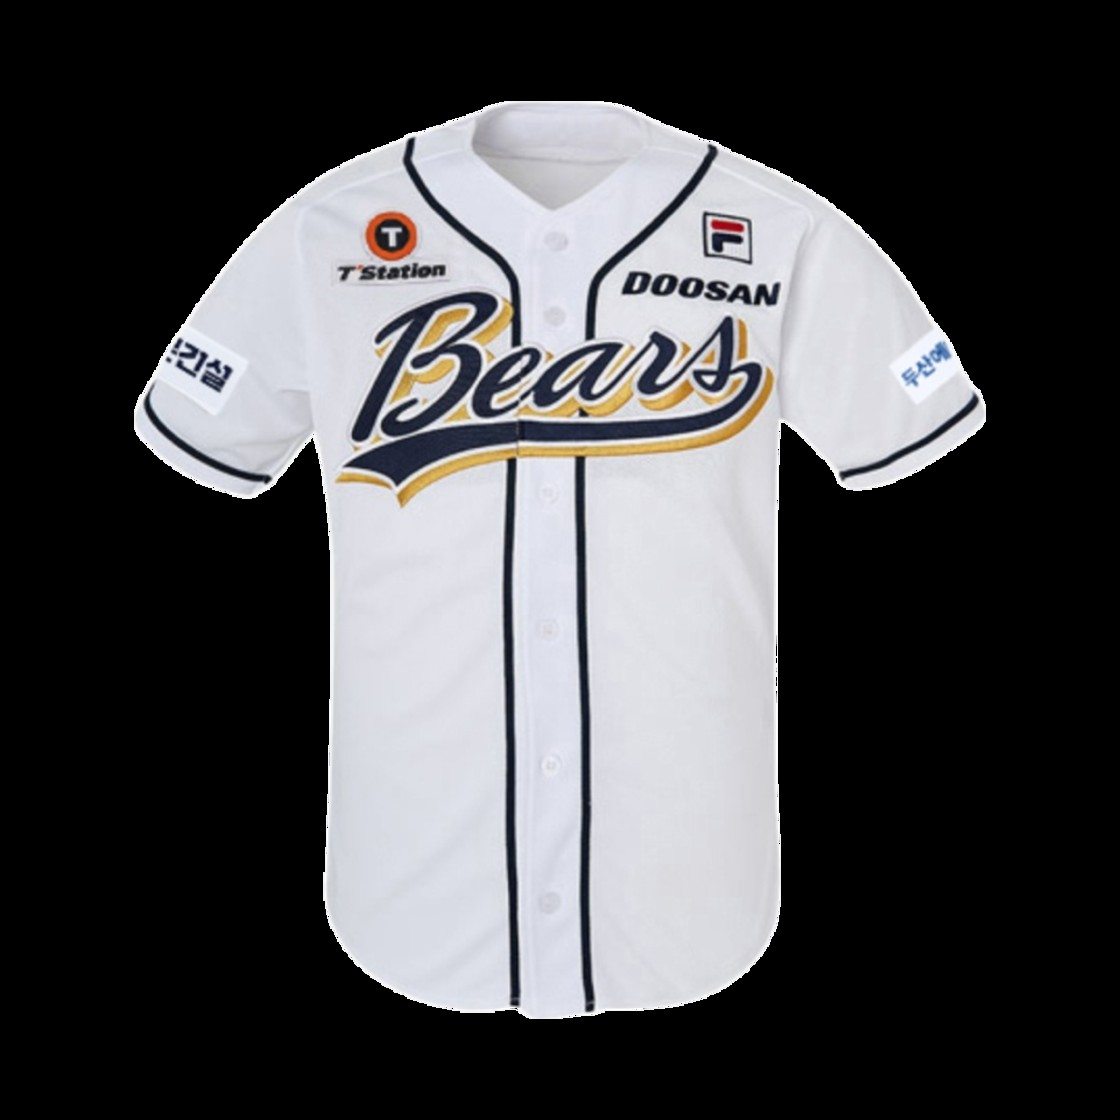
\includegraphics[width=\linewidth,height=4cm,keepaspectratio]{figures/junk_previous.jpg}\par\small 이전 시즌 유니폼 (0013.jpg)\end{minipage}
\hfill
\begin{minipage}[t]{0.31\linewidth}\centering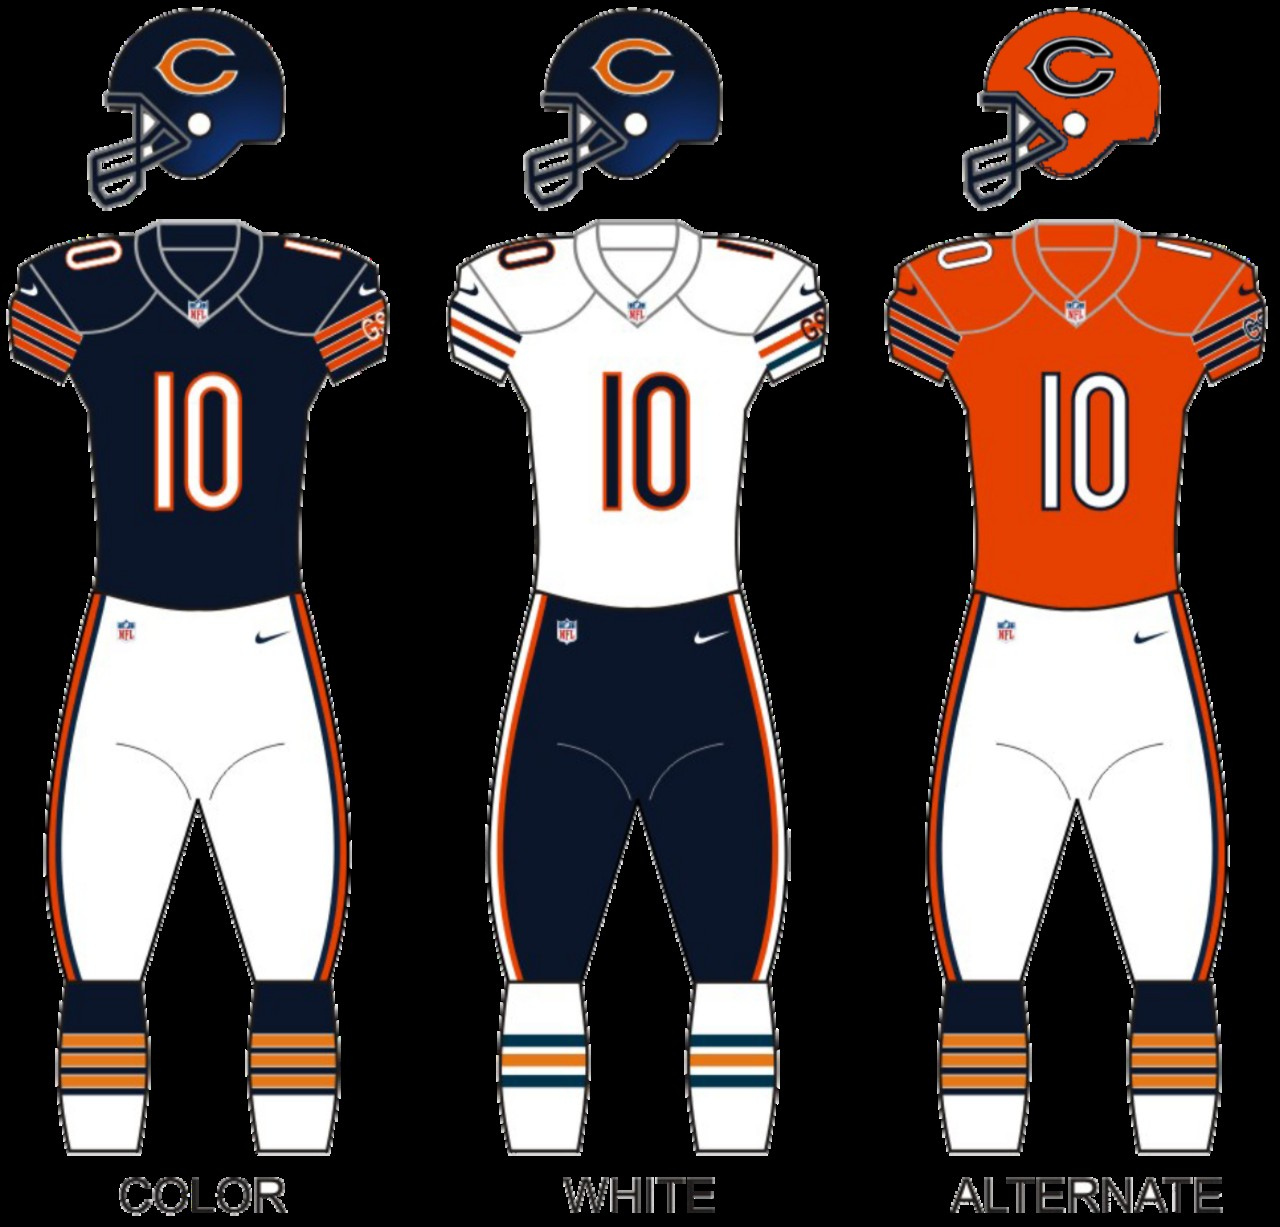
\includegraphics[width=\linewidth,height=4cm,keepaspectratio]{figures/junk_not_uniform.jpg}\par\small 유니폼 아닌 사진 (0031.jpg)\end{minipage}
\hfill
\begin{minipage}[t]{0.31\linewidth}\centering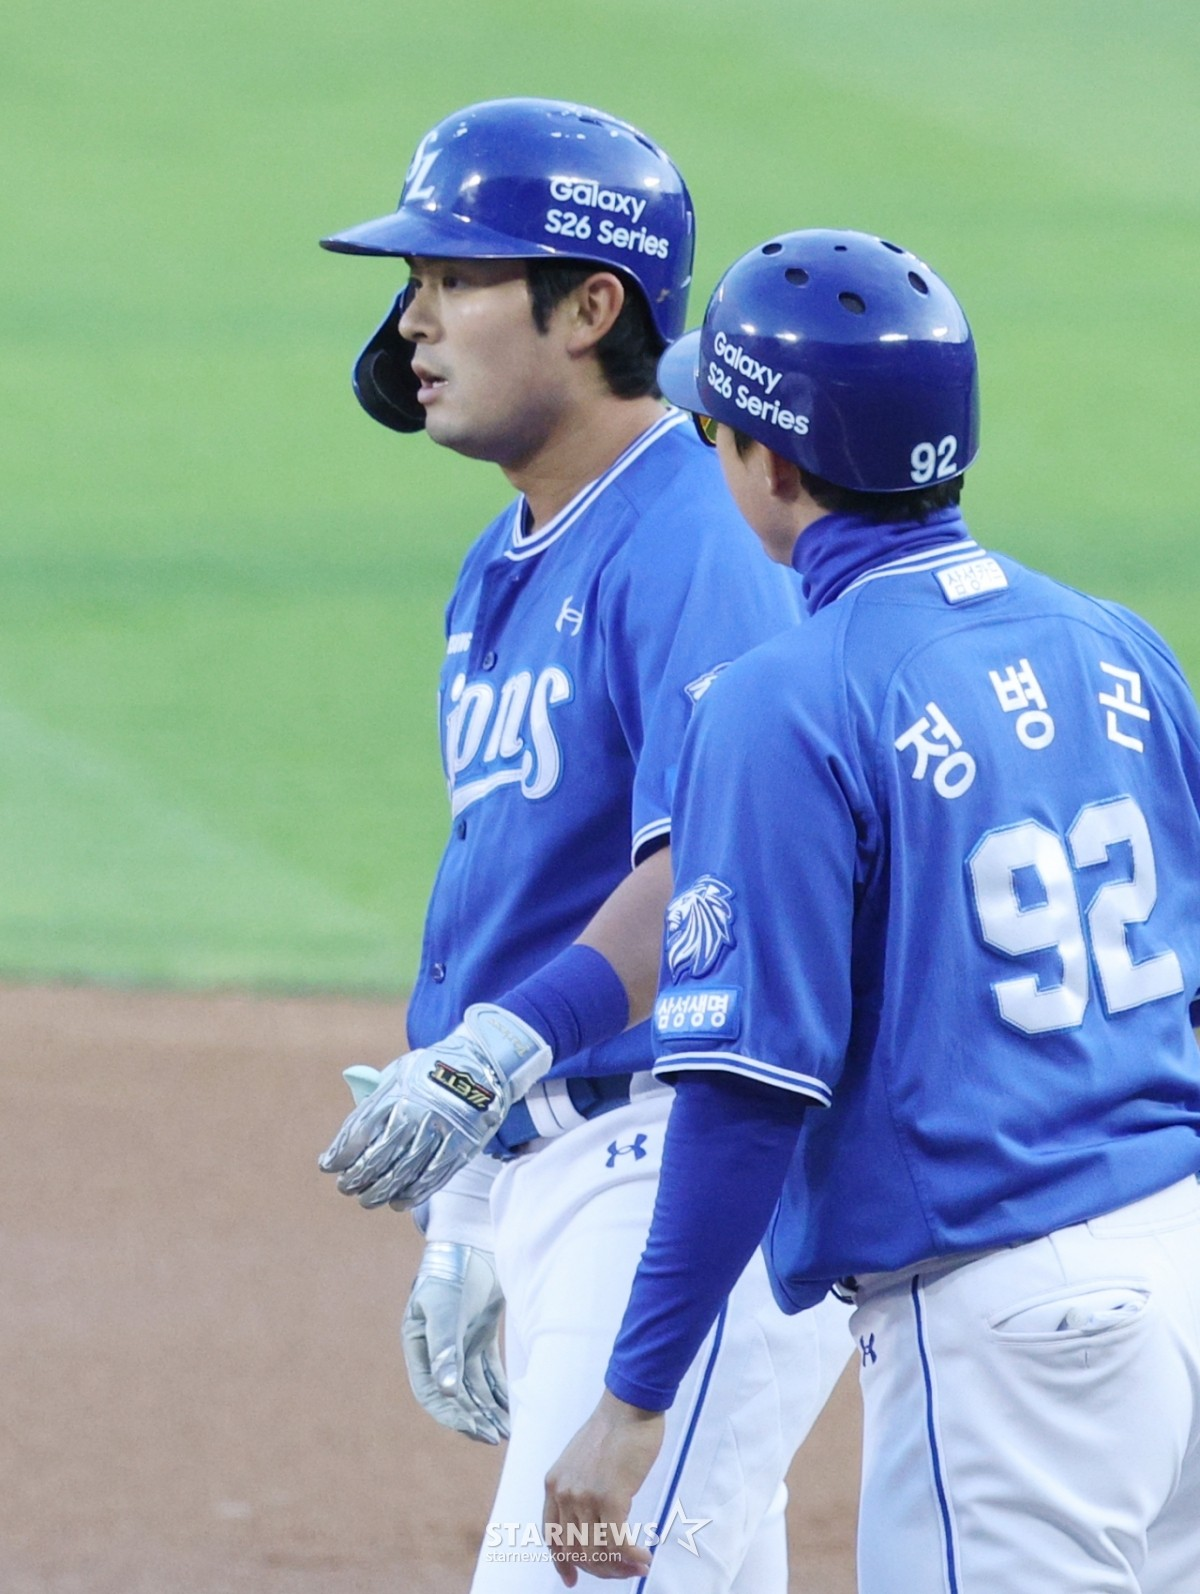
\includegraphics[width=\linewidth,height=4cm,keepaspectratio]{figures/junk_other_team.jpg}\par\small 다른 팀 유니폼 (0106.jpg)\end{minipage}

% For example: \picturefile[0.3\linewidth]{figures/junk_1.jpg}

\subsection*{What I removed}
\outputfile{outputs/clean_count.txt}

도구가 유사 사진 후보 38쌍을 제시했다. 사용자가 쌍별로 검토한 뒤 한쪽 이상이 제외된 후보는 34쌍이고, 후보 22·32·33·38은 서로 다른 각도·디자인·색상이라는 판단으로 두 장 모두 유지했다. 유사·중복 사진 사유로 이동한 고유 파일은 17장이며, 후보 쌍 수와 파일 수는 다르다. 반복된 후보에서 생긴 유지·제외 충돌은 사용자가 최종적으로 LG 0076과 한화 0063을 남기도록 지정했다.

의심 순위 상위 20장 중 최종 제외는 두산 12장, LG 9장, 한화 10장, 키움 15장이었다. 첫 육안 검토에서 이미 표시한 개수는 각각 11·6·9·15장으로, 후속 검토를 통해 상위 20장 안에서 추가 제외된 것은 각각 1·3·1·0장이었다. 상위 의심 목록 밖에서도 사용자 육안 검토에 따라 사진을 제외했다. 의심 점수만으로 자동 제외하지 않았다.
\outputfile{outputs/suspects_output.txt}
\outputfile{outputs/step12_summary.txt}
아래 내용은 사용자의 관찰 원문이며, 디자인 변경 이력·팬 규모에 관한 설명과 검색 결과의 원인 관계는 별도로 검증하지 않았다.
\outputfile{outputs/student_observations.txt}

\subsection*{Before and after cleaning}
정제 후 데이터 369장으로 학습했다. 학습 정확도는 100.0\%, 시험 정확도는 89.2\%였다. 정제 전·후 다운로드 시험 집합은 서로 달라 이 두 정확도의 차이만으로 정제 효과를 단정할 수 없다.
\picturefile{figures/clean_curves.png}
\begin{center}\picturefile[0.6\linewidth]{figures/clean_confusion.png}\end{center}
\outputfile{outputs/clean_output.txt}
\picturefile{figures/clean_worst.png}
다운로드 시험 사진 74장 중 66장을 맞혔고 오답은 8장이었다. 이 그림은 다운로드 시험 사진의 오답이며, Problem 5에서 요구하는 새로운 출처 사진의 오답을 대신하지 않는다.
\outputfile{outputs/clean_analysis_output.txt}

\outputfile{outputs/compare.txt}

\fillin{정제 후 학습 결과와 새 사진을 확보한 뒤 동일한 새 사진에서 정제 전·후 비교를 기록하기. 정제 전·후 다운로드 시험 집합은 서로 달라 정확도를 직접 비교할 때 주의하기.}

% ---------------------------------------------------------------------------
\section*{Problem 5. Images from a new source}

\fillin{Where your new images came from, and why you are sure none of them are
among your downloads.}

\outputfile{outputs/overlap.txt}

\fillin{The accuracy on your downloaded test set and on your new images, side
by side.}

\fillin{Five mistakes it was confident about, with the pictures. For each one,
what in the image you think pushed it the wrong way.}

\fillin{What is different about your new images: background, lighting, angle,
distance, what else is in the frame.}

% ---------------------------------------------------------------------------
\section*{Problem 6. The demo}

Address: \fillin{your GitHub Pages address}

\fillin{What happens when you show it something that is none of your
categories.}

% ---------------------------------------------------------------------------
\section*{Problem 7. What the model looks at}

% Copy this subsection once for every guess.
\subsection*{Guess 1}

\fillin{The guess, and what in your images or your model's mistakes made you
think of it.}

\fillin{The change you chose, and why it tests the guess.}

My request to the agent, word for word:
\begin{quote}
\fillin{the request}
\end{quote}

% One \sidebyside for every image you changed.
\sidebyside{figures/guess1_original_1.jpg}{\fillin{original: the model's answer}}
           {figures/guess1_changed_1.jpg}{\fillin{changed: the model's answer}}

\fillin{What the results say about the guess.}

\subsection*{What I now think the model uses}
\fillin{What you now think the model uses to tell your categories apart, and
how sure you are.}

% ---------------------------------------------------------------------------
\section*{Appendix. Output of check.py}
\outputfile{outputs/check.txt}

\end{document}
